% Тип документа
\documentclass[a4paper,12pt]{extarticle}

% Шрифты, кодировки, символьные таблицы, переносы
% \usepackage{cmap}
% \usepackage[T2A]{fontenc}
\usepackage[utf8]{inputenc}
\usepackage[russian]{babel}
% Это пакет -- хитрый пакет, он нужен но не нужен
\usepackage[mode=buildnew]{standalone}

\usepackage
	{
		% Дополнения Американского математического общества (AMS)
		amssymb,
		amsfonts,
		amsmath,
		amsthm,
		% Пакет для физических текстов
		physics,
		% misccorr,
		% 
		% Графики и рисунки
		wrapfig,
		graphicx,
		subcaption,
		float,
		tikz,
		tikz-3dplot,
		caption,
		csvsimple,
		color,
		booktabs,
		geometry,
		% 
		% Таблицы, списки
		makecell,
		multirow,
		indentfirst,
		%
		% Интегралы и прочие обозначения
		ulem,
		esint,
		esdiff,
		% 
		% Колонтитулы
		fancyhdr,
	} 
    
\usepackage{mathtools}
% \mathtoolsset{showonlyrefs=true} 
\usepackage{pgfplots,pgfplotstable,booktabs,colortbl}
\usepackage{xcolor}
\usepackage{hyperref}
\usepackage{pythontex}
 % Цвета для гиперссылок
\definecolor{linkcolor}{HTML}{000000} % цвет ссылок
\definecolor{urlcolor}{HTML}{799B03} % цвет гиперссылок
 
\hypersetup{pdfstartview=FitH,linkcolor=linkcolor,urlcolor=urlcolor, colorlinks=true}
\hypersetup{pageanchor=false}
% Увеличенный межстрочный интервал, французские пробелы
\linespread{1.1} 
\frenchspacing 

\newcommand{\mean}[1]{\langle#1\rangle}

\begin{pycode}
##
def frexp10(decimal):
	parts = ('%e' % decimal).split('e')
	return float(parts[0]), int(parts[1])
##
\end{pycode}



% Функция для тех, кто использует pythontex. Представляет любое вещественное число в стандартном виде.
\newcommand{\frexp}[1]{
		\pyc{#10=frexp10(#1)} 
			\py{ round(#10[0],2)} 
				\cdot 10^{\py{#10[1]}} }

% const прямым шрифтом
\newcommand\ct[1]{\text{\rmfamily\upshape #1}}
\newcommand*{\const}{\ct{const}}
\usepackage{array}
\usepackage{pstool}

\geometry		
	{
		left			=	2cm,
		right 			=	2cm,
		top 			=	2.5cm,
		bottom 			=	2.5cm,
		bindingoffset	=	0cm
	}

%%%%%%%%%%%%%%%%%%%%%%%%%%%%%%%%%%%%%%%%%%%%%%%%%%%%%%%%%%%%%%%%%%%%%%%%%%%%%%%
	%применим колонтитул к стилю страницы
%\pagestyle{fancy} 
	%очистим "шапку" страницы
% \fancyhead{} 
	%слева сверху на четных и справа на нечетных
%\fancyhead[R]{}%\labauthors 
	%справа сверху на четных и слева на нечетных
% \fancyhead[L]{Отчёт по лабораторной работе №\labnumber}
%\fancyhead[L]{\labtheme} 
	%очистим "подвал" страницы
% \fancyfoot{} 
	% номер страницы в нижнем колинтуле в центре
\fancyfoot[C]{\thepage} 

%%%%%%%%%%%%%%%%%%%%%%%%%%%%%%%%%%%%%%%%%%%%%%%%%%%%%%%%%%%%%%%%%%%%%%%%%%%%%%%

\renewcommand{\contentsname}{Оглавление}
\usepackage{tocloft}
\usepackage{secdot}
\sectiondot{subsection}


\begin{document}
\def\labauthor{Есюнин Д.В.}
\def\labgroup{0420ДМР1Г}
\def\labtheme{Исследование динамики мембранного потенциала нейрона под воздействием щума с помощью уравнения Фоккера-Планка}
%!TEX root = ../diplom.tex
\newgeometry{left=30mm,right=15mm,top=15mm,bottom=25mm,bindingoffset=0cm,headheight=15pt}
\begin{titlepage}
%\begin{spacing}{1}
	\fontsize{13pt}{13pt} \selectfont
	{\centering
	\linespread{1}
	\noindent{\fontsize{11pt}{11pt}\textbf{ МИНИСТЕРСТВО НАУКИ И ВЫСШЕГО ОБРАЗОВАНИЯ РОССИЙСКОЙ} \\[0.2em]  \textbf{ ФЕДЕРАЦИИ}}\\[13pt]
%	\begin{spacing}{1.5}
		{\fontsize{13pt}{13pt} \selectfont\bf  Федеральное государственное автономное образовательное учреждение \\
		высшего образования \\
		<<Национальный исследовательский \\ Нижегородский
		государственный университет им. Н.И. Лобачевского>>
		}\\[12pt] 
%	\end{spacing}
	{\fontsize{13pt}{13pt} \selectfont
	Радиофизический факультет\\
	Кафедра теории колебаний и автоматического регулирования\\[28pt]
	Направление <<Радиофизика>>\\
	\vspace{30pt}
	ОТЧЕТ ПО УЧЕБНОЙ ПРАКТИКЕ\\}
	\vspace{15pt}
	{\fontsize{15pt}{15pt}
	Практика по получению первичных профессиональных\\
	умений и навыков
	\vspace{15pt}
	}\\
	{\fontsize{13pt}{13pt}
		НАЗВАНИЕ ОТЧЕТА
	}\\
	\vspace{48pt}}\fontsize{12pt}{12pt} \selectfont
	\noindent
	Научный руководитель:\\[0.4em]
	доцент, к.ф.-м.н.,\hfill \rule{2cm}{1pt} Клиньшов В.В. \hphantom{,}\\[40pt]
	%
	%
	Научный консультант:\\[0.4em]
	ученая степень, звание\hfill \rule{2cm}{1pt} ФИО\hphantom{aaaaaaaaaa,}\\[50pt]
	%
	%
	Студент 1-го курса магистратуры:
	\hfill \rule{2cm}{1pt} Есюнин Д.В. \hphantom{aa,}\\[30pt]
	\vfill
	\centering
	Нижний Новгород\\[0.4em]
	2020 год
% \noindent\tikz[remember picture,overlay] {
% % % \draw[draw=none,fill=black!50!gray]  rectangle ;
% % \draw [step=1.0cm,gray] (current page.north east) grid (current page.south west);
% \node[opacity=1,inner sep=0pt] at (current page.center){\includegraphics[width=\paperwidth,height=\paperheight]{fig/apt.png}
% };}
%\end{spacing}
\end{titlepage}
\clearpage
\restoregeometry
\newpage
\renewcommand{\phi}{\varphi}
\renewcommand{\div}{\text{div}}
\renewcommand{\grad}{\text{grad}}

\section*{Введение}
В больших нейронных сетях, где имеется огромное количество нейронов, организованных в сети функционально сходных нейронов. Типичный кортикальный нейрон получает тысячи синапсов, большинство из них от соседних нейронов; воздействие одного пресинаптического спайка на постсинаптическую клетку относительно невелико. Более того, спайковые цепочки кортикальных нейронов в высшей степени стохастичны и нерегулярны, следовательно, существует много шума в синхронизации спайков. Возникает вопрос о том, передает ли наблюдаемая нерегулярность последовательности спайков информацию или, скорее, отражает влияние различных источников шума, присутствующих в клетке. Даже если время межспайковых интервалов от отдельных клеток зашумлено, информация все равно может передаваться в средней активности слабо коррелированных нейронов. 

\textbf{Целью} работы является исследование динамики нейрона под воздействием шума с помощью уравнения Фоккера-Планка. Полученные характеристики выходного сигнала позволят в дальнейшем изучить возникающие режимы в больших нейроны сетях.
\section{Модель нейрона <<накопление и сброс>>}
Для описания динамики нейронов применяются модели разного уровня сложности. Одна из простейших моделей нейрона «накопление и сброс». Эта система описывается следующим дифференциальным уравнением:
\begin{equation}
	C_m\frac{dV(t)}{dt}=-g_L(V(t)-V_L)+I(t)
	\label{eq:1}
\end{equation}
Разность напряжений $V(t)$ на мембране изменяется в
ответ на инжектируемый ток $I(t)$, $C_m=0.2 нФ$ - емкость мембраны, $g_L=20 нСм$ - проводимость утечки, $V_L$ - потенциал покоя. Согласно модели "накопление и сброс" нейрон рассматривается как $RC$-цепь с постоянной времени
\begin{equation}
	\tau_m=\frac{C_m}{g_L}=10 \text{мс}
	\label{eq:2} 
\end{equation}
Генерация спайка происходит в момент достижения мембранного потенциала порогового напряжения $V_\text{th}$ таким образом, что нейрон, как говорят, испускает спайк в момент времени $t_\text{spk}$ всякий раз, когда 
$V(t=t_\text{spk})=V_\text{th} =-50 \text{ мВ}$, после чего его потенциал мгновенно приобретает значение $U_r=-60 \text{ мВ}$. После этого система находится в состоянии сброса $U_r$ в течение времени рефрактерности $\tau_r=2 \text{ мс}$, затем вновь начинает эволюционировать в соответствие с уравнением \eqref{eq:1}. $I(t)$ представляет собой общий синаптический ток, который равен линейной сумме вкладов каждой отдельной пресинаптической клетки.

Начнем с простейшего описания взаимодействия между пре- и пост-синаптическими нейронами. Это сводится к предположению, что каждый пресинаптический спайк вызывает мгновенное изменение постсинаптического напряжения, которое не зависит от текущего значения этого напряжения и зависит только от параметра $J$, измеряющего силу синапса. Если $C$ синапсов идут на нейрон, с величиной связи $J_i (i=1,\ldots,C)$, то ток, поступающий в клетку может быть представлен как
\begin{equation}
	I(t)=\sum_{i}^{C}J_i\sum_{j}\delta(t-t_j^i)
	\label{eq:3}
\end{equation}
где $t_i^j$ - время $j$-го спайка от $i$-го пресинаптического нейрона. Если нейрон изначально находится в состоянии покоя, а пресинаптическая клетка запускает одиночный cпайк в момент времени $t=0$, то путем
интегрирования уравнения \eqref{eq:1} получается
\begin{equation}
	V(t)=V_L+\frac{J_i}{C_m}exp(-\frac{t}{\tau_m})\Theta(t)
	\label{eq:4}
\end{equation}

Мы рассматриваем нейрон, получающий синаптический вход от большого числа возбуждающих и тормозящих клеток. Мы делаем два важных предположения относительно активности этих входов: во-первых, каждый из них генерирует спайки в соответствии со стационарным процессом Пуассона, то есть с постоянной вероятностью испускания спайка в единицу времени. Во-вторых,
эти пуассоновские процессы независимы от клетки к клетке, то есть возникновение спайка из любой данной клетки не дает никакой информации о вероятности срабатывания любого другого нейрона. Эти предположения необходимо будет проверить на сетевом уровне чтобы теория была самосогласованной.

Обозначим частоту срабатывания возбуждающих (тормозящих) нейронов, как $\nu_{E_j} (\nu_{I_j})$, а величину воздействия соответствующих возбуждающих (тормозящих) синапсов, как $J_{E_j} (J_{I_j})$. Для простоты мы сначала предположим, что все частоты срабатывания и величины воздействия из каждой пресинаптической популяции идентичны, т. е. $\nu_{E_j}=\nu_{E} \text{ и } J_{E_j}=J_{I}$ для всех $j$
и аналогично для тормозящих нейронов. В этой простой ситуации среднее значение общего тока по времени является постоянным во времени и задается
\begin{equation}
	<I(t)>=\mu_C=\sum_{j=1}^{C_E}J_{E_j}\nu_{E_j}-\sum_{j=1}^{C_I}J_{I_j}\nu_{I_j}=C_EJ_E\nu_{E}-C_IJ_I\nu_{I}
	\label{eq:5}
\end{equation}
Для процесса Пуассона $s(t)$ с интенсивностью $\nu$ $<s(t)-\nu)(s(t')-\nu)>=\nu\delta(t-t')$. Таким образом,
используя тот факт, что входы являются Пуассоновскими и независимыми, связанная корреляционная функция полного тока задается
\begin{equation}
\begin{split}
		<(I(t)-<I>)(I(t')-<I>)> &
	=\left[\sum_{j=1}^{C_E}J^2_{E_j}\nu_{E_j}-\sum_{j=1}^{C_I}J^2_{I_j}\nu_{I_j}\right]\delta(t-t')= \\
	=[C_EJ^2_E\nu_{E}-C_IJ^2_I\nu_{I}]\delta(t-t')=\sigma_C^2\delta(t-t')
	\label{eq:6}
\end{split}
\end{equation}

\section{Численное решение уравнения Фоккера-Планка}
Поскольку входы в нейрон считаются стохастическими, временная эволюция
$V(t)$ является вероятностной. Фундаментальным объектом для описания динамики мембранного потенциала является плотность вероятности $\rho(V, t|V_0, t_0)$ для $V(t)\in[V, V+dV]$ учитывая, что $V(t_0)=V_0$. Если мы рассмотрим ансамбль одинаковых нейронов с разным реализациями, то $\rho(V, t|V_0, t_0)$ - это доля нейронов в ансамбле с мембранным потенциалом $[V, V+dV]$, учитывая, что все нейроны находились в $V_0$ при $t=t_0$. Уравнение, описывающее динамику функции $\rho(V, t|V_0, t_0)$ называется уравнением Фоккера-Планка.
\begin{equation}
%\begin{split}
\frac{\partial \rho(V, t|V_0, t_0)}{\partial t}=
\frac{\partial }{\partial V}\left[\frac{V-V_{ss}}{\tau_m}\rho(V, t|V_0, t_0)\right]+\frac{\sigma_V^2}{2\tau_m}\frac{\partial^2 }{\partial V^2}\left[\rho(V, t|V_0, t_0)\right]
%\end{split}
\label{eq:7}
\end{equation}
Для решения уравнения в частных производных будем использовать метод сеток. Рассмотрим отрезок $[V_L, V_{th}]$ и разобьем его на $n$ частей с шагом $\displaystyle h=\frac{V_L- V_{th}}{n}$. Поскольку $\rho(V_{th}, t|V_0, t_0)=0$, плотность вероятности должна быть равна нулю при $V=V_{th}$, в противном случае производная по напряжению была бы бесконечной при $V=V_{th}$. Поэтому мы имеем следующие граничные условия 
\begin{equation}
	\rho(V_{th}, t|V_0, t_0)=0 \qquad \text{ и } \qquad \frac{\partial }{\partial V}\rho(V, t|V_0, t_0)=-\frac{2\nu(t)\tau_m}{\sigma_V^2}
	\label{eq:8}
\end{equation}
Условия того, что плотность вероятности исчезает
достаточно быстро при $V\to-\infty$, дает дополнительные условия на левой границе
\begin{equation}
	\lim\limits_{V\to V_L}\rho(V, t|V_0, t_0)=0 \qquad \text{ и } \qquad \lim\limits_{V\to V_L}V\rho(V, t|V_0, t_0)=0
	\label{eq:9}
\end{equation}
Перейдем от уравнения в частных производных к системе уравнений в полных производных по времени. Для этого заменим производные по напряжению в уравнении \eqref{eq:7} на разностные суммы:
\begin{equation}
\begin{split}
	\frac{\partial \rho(V, t|V_0, t_0)}{\partial V}=\frac{\rho_{i+1}-\rho_{i}}{2h} \\
	\frac{\partial^2 \rho(V, t|V_0, t_0)}{\partial V^2}=\frac{\rho_{i+1}-2\rho_{i}+\rho_{i-1}}{h^2}
	\label{eq:10}
\end{split}
\end{equation}
Тогда уравнение Фоккера-Планка примет вид:
\begin{equation}
\begin{cases}
\rho_1=0 \\
\displaystyle \frac{d\rho_{i}}{dt}=\frac{V_i-V_{ss}}{2\tau_m}\cdot\frac{\rho_{i+1}-\rho_{i}}{2h}+\frac{\rho_{i}}{\tau_m}+\frac{\sigma_V^2}{2\tau_m}\cdot\frac{\rho_{i+1}-2\rho_{i}+\rho_{i-1}}{h^2}\\
.\\
.\\
.\\
\rho_n=0
\end{cases}
\label{eq:11}
\end{equation}
Первоначально все нейроны в ансамбле находятся в состоянии $V(0)=V_r$. Тогда условная плотность вероятности принимает вид $\rho(V, t_0|V_0, t_0)=\delta(V-V_r)$. Метод сеток для решения уравнения Фоккера-Планка устойчив только в том случае, если начальное распределение условной плотности вероятности имеет ширину, сравнимую с величиной шага $h$.

Известно, что фундаментальным решением уравнения Фоккера-Планка в случае начального распределения в виде дельта-функции является нормальное распределение вида
\begin{equation}
	\rho(V,t)=\frac{1}{\sqrt{2\pi D_V(t)}}exp\left(-\frac{(V(t)-V_{mean}(t)}{2D_V(t)}\right)
\label{eq:12}
\end{equation}
Где $V_{mean}(t)$ - среднее значение условной плотности вероятности, а $D_V(t)$ - ее дисперсия.

Рассмотрим уравнение \eqref{eq:7} и введем коэффициенты $a(V)=\frac{V_{ss}}{\tau_m}$, $b(V)=\frac{\sigma_V^2}{\tau_m}$. Разложим коэффициенты $a(V), b(V)$ в окрестности $V=V_{mean}$ до первого слагаемого
\begin{equation}
a(V)\approx a(V_{mean})+a'(V_{mean})(V-V_{mean}), \qquad b(V)\approx b(V_{mean})
\label{eq:13}
\end{equation}

Подставив \eqref{eq:13} в уравнение \eqref{eq:7} и приравняв члены при одинаковых степенях разности $V-V_{mean}$ получим систему из двух обыкновенных дифференциальных уравнений
\begin{equation}
\begin{cases}
\displaystyle \frac{dV_{mean}}{dt}=\frac{V_{ss}-V_{mean}}{\tau_m} \\
\displaystyle \frac{dD_V}{dt}=2D_Va'(V_{mean})+b(V_{mean})
\end{cases}
\label{eq:14}
\end{equation}
Таким образом получим выражение для смещения центра $\displaystyle V_{mean}=V_{ss}-(V_{ss}-V_r)e^{-\frac{t}{\tau_m}}$ и ширины условной плотности вероятности $\displaystyle \sigma(t)=\frac{\sigma_V}{\sqrt{2}}\left[1-e^{-\frac{2t}{\tau_m}}\right]^{1/2}$

Определим время $t'$, когда СКО сравнимо с шагом сетки $\sigma(t')=ch$, где $c=1,2,\ldots$
\begin{equation}
	ch=\frac{\sigma_V}{\sqrt{2}}\left[1-e^{-\frac{2t'}{\tau_m}}\right]^{1/2}
	\label{eq:15}
\end{equation}

Решая это уравнение получим $\displaystyle t'=\frac{\tau_m}{2}ln\frac{1}{1-\frac{2c^2h^2}{\sigma_V^2}}$

В таком случае можно задать распределение условной плотности вероятности через момент времени $t'$ в виде нормального распределения с заданным средним и дисперсией. Мы должны рассматривать достаточно малый интервал времени $t'$, чтобы не учитывать наличие поглощающего барьера на границе $V=V_{th}$, то есть нужно полагать, что хвост гауссова распределения в точке $V=V_{th}$ меньше погрешности решения системы уравнений \eqref{eq:11}.

Численное решение системы уравнений \eqref{eq:11} было найдено с помощью метода Рунге-Кутта 5 порядка при использовании встроенной функции ode45 в среде Matlab. Вид условной плотности вероятности в разные моменты времени представлен на рис. \ref{pic:1}.
\begin{figure}[H]
	\centering
	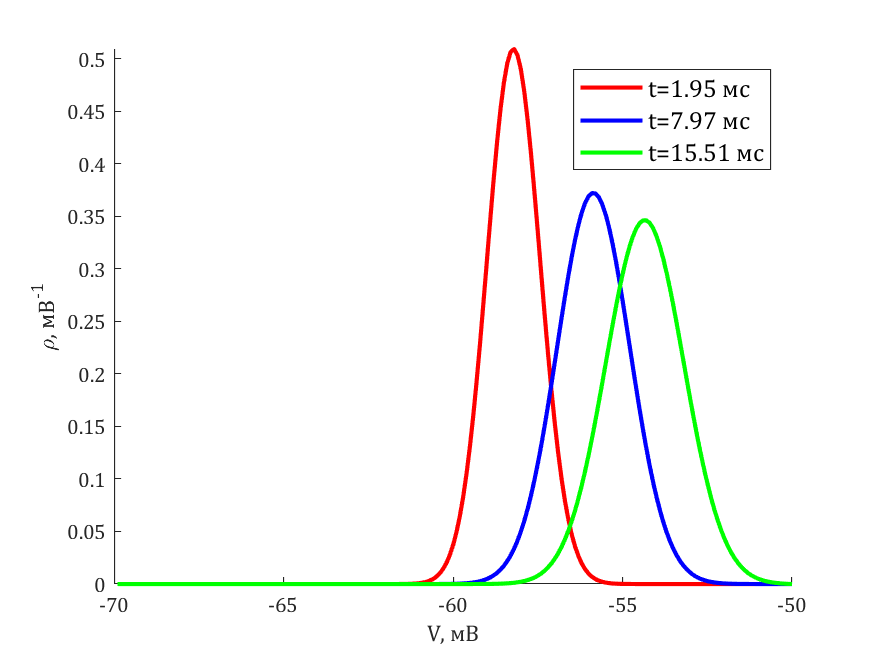
\includegraphics[width=\linewidth]{pic/rho.png}
	\caption{Условная плотность вероятности $\rho(V,t)$  в разные моменты времени}
	\label{pic:1}
\end{figure}

Введем функцию потока вероятности $\displaystyle S(t)=\int_{V_L}^{V_{th}}\rho(V,t)dV$, которая характеризует вероятность нахождения мембранного потенциала к моменту времени $t$ в интервале $V\in[V_L, V_{th}]$. В таком случае функция $1-S(t)$ характеризует вероятность срабатывания нейрона к моменту времени $t$, то есть является интегральной функцией распределения межспайкового интервала. Продифференцировав это выражение по $t$ получим условную плотность вероятности межспайкового интервала для ансамбля частиц. Вид этой функции представлен на рис. \ref{pic:2}.
\begin{figure}[H]
	\centering
	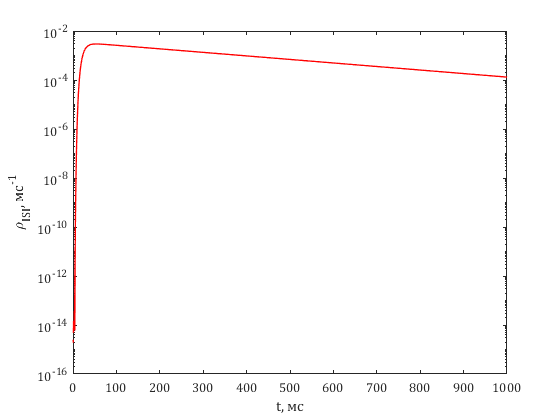
\includegraphics[width=\linewidth]{pic/S.png}
	\caption{Условная плотность вероятности межспайкового интервала $\rho_{ISI}(t)$}
	\label{pic:2}
\end{figure}
\section{Cравнение решения уравнения Фоккера-Планка с микроскопической системой}
Поскольку уравнение Фоккера-Планка описывает условную плотность вероятности нахождения мембранного потенциала клетки в интервале $V\in[V_L, V_{th}]$ для большого числа частиц, то необходимо сравнить распределения, получаемые в результате численного решения уравнения ФП, с распределениями, получаемыми в результате моделирования большого числа нейронов $N$. Ансамбль, состоящий из $N$ таких нейронов, называется микроскопической системой.

Для того, чтобы найти условную плотность вероятности $\rho(V,t)$ для этой системы, необходимо промоделировать динамику $N$ нейронов под воздействием белого шума с заданными характеристиками $\mu_C=g_L(V_{ss}-V_L)$ и $\sigma=\sigma_V$. 
График зависимости условной плотности вероятности в фиксированный момент времени представлен на рис. \ref{pic:3}.
\begin{figure}[H]
	\centering
	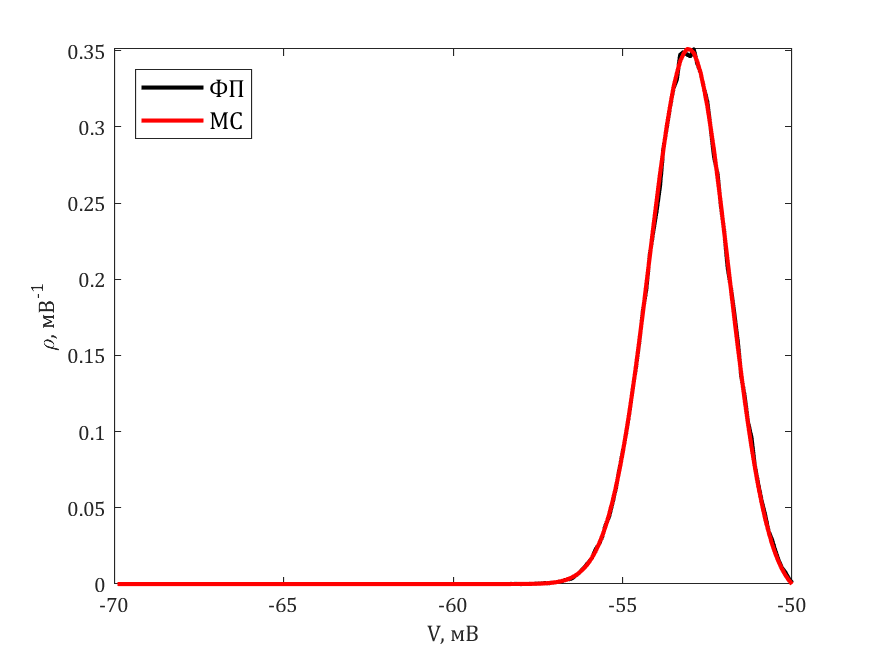
\includegraphics[width=\linewidth]{pic/rhomicro.png}
	\caption{Условная плотность вероятности $\rho(V,t)$ при численном решении уравнения ФП и для микроскопической системы (МС) в момент времени $t=15\text{ мс}$}
	\label{pic:3}
\end{figure}
Чтобы определиться с числом нейронов, которые необходимо выбрать в микроскопической системе, необходимо проанализировать зависимость относительной ошибки распределений в случае решения уравнения ФП и микроскопической системы $\epsilon(N)$ от числа нейронов в системе $N$. График зависимости $\epsilon(N)$ представлен на рис. \ref{pic:4}. Очевидно, что при $N\to\infty$ относительная ошибка будет стремиться к нулю, но на программном уровне нельзя выбрать сколько угодно большое число $N$, так как это приводит к неограниченному росту времени симуляции. В качестве значения числа нейронов в системе мы остановились на величине $N=10^6$.
\begin{figure}[H]
	\centering
	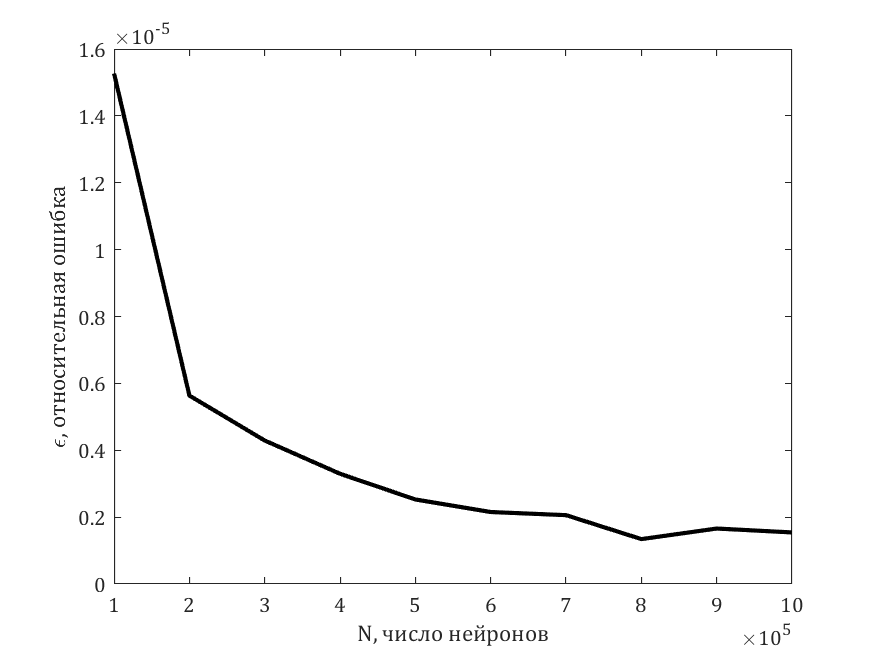
\includegraphics[width=\linewidth]{pic/epsilonN(N).png}
	\caption{Относительная ошибка $\epsilon(N)$ от числа нейронов в микроскопической системе $N$}
	\label{pic:4}
\end{figure}

При фиксированном числе нейронов в микроскопической системе стоит также следить за количеством ячеек по напряжению $n$. Так как с одной строны шаг ячейки должен быть мал по сравнению со всем интервалом напряжений $h<<\Delta V$, но с другой строны в одну ячейку должно попадать большое число нейронов из микроскопической системы $\frac{N}{n}>>1$. Из этих условий получим ограничение на количество ячеек в интервале напряжений $1<<n<<N$. В качестве оптимального значения $n$ выберем среднее геометрическое из левой и правой границы неравенства $n=\sqrt{N}$. Проанализируем зависимость относительной ошибки $\epsilon(n)$ от количества ячеек в интервале напряжений $n$. График $\epsilon(n)$ представлен на рис. \ref{pic:5}
\begin{figure}[H]
	\centering
	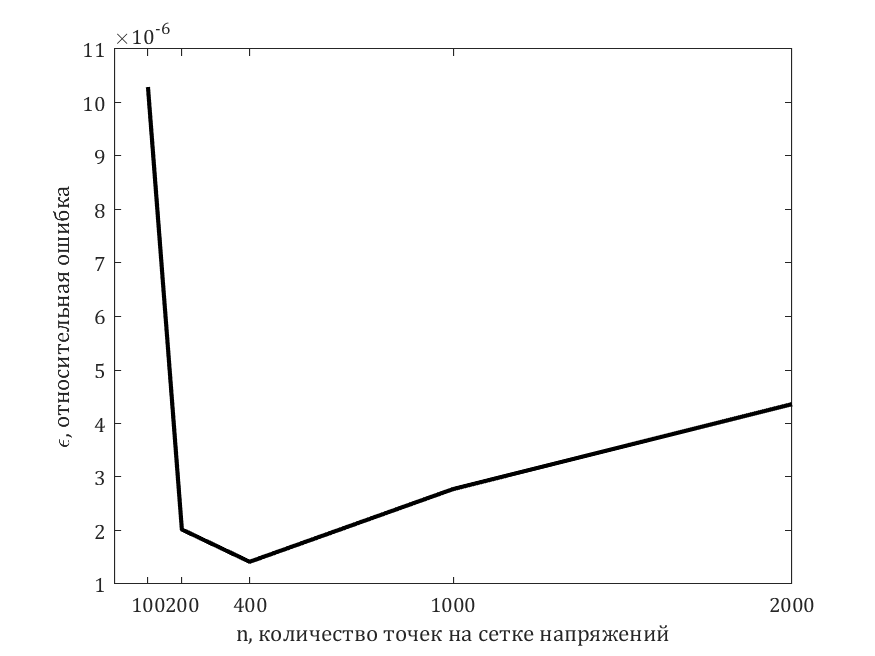
\includegraphics[width=\linewidth]{pic/epsilon(n).png}
	\caption{Относительная ошибка $\epsilon(n)$ от числа ячеек в интервале напряжений $n$}
	\label{pic:5}
\end{figure}

\section{Анализ области параметров входного сигнала}
Так как следующей задачей в данной работе является анализ характеристик сети, состоящей из большого числа нейронов, то необходимо проанализировать динамику одного нейрона в зависимости от характеристик входного сигнала. Каждый нейрон в связанной сети получает на входе сигнал с определенными характеристиками, под действием которого генерирует выходной сигнал, характеристики которого определяются характеристиками входного сигнала. Однако в сети выходные сигналы с нейронов складываются и вновь подаются на их вход, поэтому характеристики входного сигнала также зависят от характеристик выходного сигнала. Мы полагаем, что на вход клетки поступает пуассоновский поток событий, в таком случае выходным сигналом также должен являться сигнал с распределением Пуассона для большой сети. В таком случае фактор Фано должен стремиться к единице $\displaystyle f=\frac{<T_{ISI}>}{\sigma(T_{ISI})}\to 1$. Рассмотри два режима работы нейрона:
\paragraph{Область регулярного срабатывания нейронов}

Будем полагать, что начальное распределение плотности вероятности является $\delta$-функцией в точке $V_r$. Рассмотри решение уравнения Фоккера-Планка в отсутствии границы. Тогда ширина $\Delta V$ условной плотности вероятности в момент, когда ее центр проходит точку $V_{th}$ должна быть много меньше $\displaystyle \lim\limits_{t\to\infty}\sigma(t)=\frac{\sigma_V}{\sqrt{2}}\left[1-e^{-\frac{2t}{\tau_m}}\right]^{1/2}=\Delta V_{ss}=\frac{\sigma_V}{\sqrt{2}}$, то есть $\displaystyle \Delta V<<\frac{\sigma_V}{\sqrt{2}}$
Используя уравнение \eqref{eq:14} можно найти ширину $\displaystyle \Delta V=\sigma(t)=\frac{\sigma_V}{\sqrt{2}}\left[1-\left(\frac{V_{th}-V_{ss}}{V_r-V_{ss}}\right)^2\right]^{1/2}$. Регулярное срабатывание означает, что СКО межспайкового интервала должно быть много меньше среднего значения $\Delta T_{ISI}<<T_{ISI}$, тогда $\displaystyle\Delta T_{ISI}=\frac{\Delta V}{\dot{V}|_{t=T_ISI}}<<T_{ISI}$. В итоге получим ограничение на эту область
\begin{equation}
\frac{\sigma_V}{\sqrt{2}}\left[1-\left(\frac{V_{th}-V_{ss}}{V_r-V_{ss}}\right)^2\right]^{1/2}<<(V_{ss}-V_{th})ln\frac{V_r-V_{ss}}{V_{th}-V_{ss}}
\label{eq:16}
\end{equation}
\paragraph{Область редкого срабатывания нейронов}
Будем также полагать, что начальное распределение плотности вероятности является $\delta$-функцией в точке $V_r$. В таком случае достижение этого режима возможно, если $\Delta V_{ss}<<V_{th}-V_{ss}$, то есть будет справедливо следующее соотношение 
\begin{equation}
\frac{\sigma_V}{\sqrt{2}}<<V_{th}-V_{ss}
\label{eq:17}
\end{equation}

На рис. \ref{pic:6} представлено разбиение пространства параметров на области, описываемые уравнениями \eqref{eq:16} и \eqref{eq:17}, где  неравенство $<<$ переходит в уравнение $=$. На диаграмме также представлены значения Фано-фактра в зависимости от интенсивности шума $\sigma_V$ и постоянного воздействия $\mu_C$.
\begin{figure}[H]
	\centering
	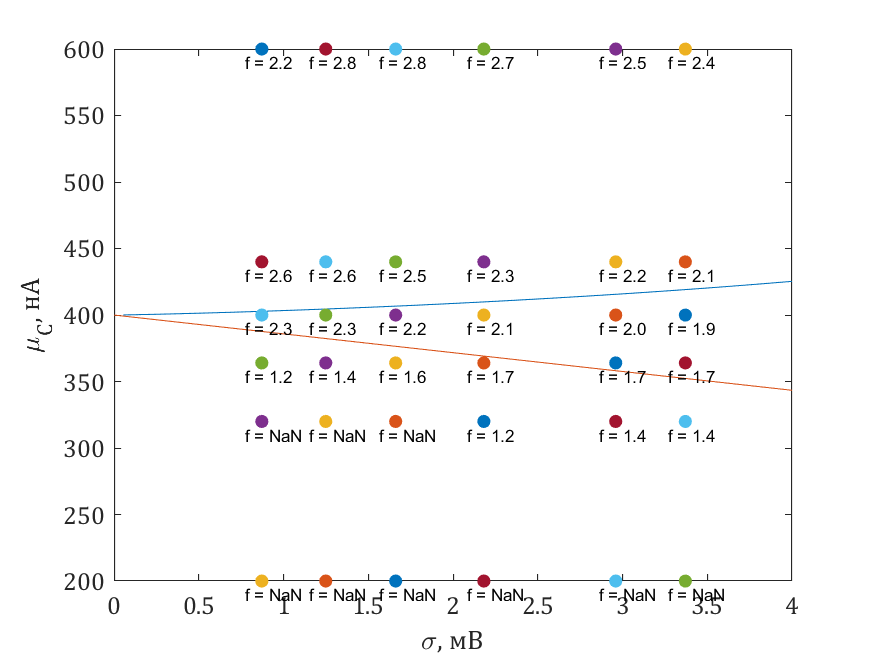
\includegraphics[width=0.8\linewidth]{pic/T_mean_T_sigma3.png}
	\caption{Область параметров внешнего воздействия}
	\label{pic:6}
\end{figure}
\section*{Заключение}
В данной работе было рассмотрено численно решение уравнение Фоккера-Планка для условной плотности вероятности $\rho(V, t|V_0, t_0)$. Было показано, что распределения, полученные в результате решения уравнения \eqref{eq:7}, имеют хорошее соответствие с распределениями в микроскопической системе. Этот факт позволяет в дальнейшем рассматривать коллективную динамику сети на основе уравнения ФК, а не микроскопического распределения, что значительно сильно экономить временные ресурсы на моделирование сети.
\end{document}